\documentclass[10pt,a4paper]{article}
\usepackage[utf8]{inputenc}
\usepackage[T1]{fontenc}

% graphics and color housekeeping
\usepackage{graphicx}
\usepackage[usenames, dvipsnames]{xcolor}
\usepackage{float}

% nicer math
\usepackage{mathtools}
\usepackage{amsmath}
\usepackage{amsfonts}
\usepackage{amsthm}
\usepackage{thmtools}
\usepackage{cancel}


% nice indicator function
%% https://tex.stackexchange.com/questions/26637/how-do-you-get-mathbb1-to-work-characteristic-function-of-a-set
\usepackage{bbm}

\usepackage{enumitem}
\newtheorem{theorem}{Theorem}[section]
\newtheorem{lemma}[theorem]{Lemma}
\newtheorem*{claim}{Claim}
\newtheorem{corollary}[theorem]{Corollary}

\theoremstyle{remark}
\newtheorem*{remark}{Remark}

\theoremstyle{definition}
\newtheorem{definition}{Definition}[section]
\newtheorem{subdefinition}{Definition}[definition]

\declaretheorem[sibling=definition, shaded={rulecolor=black, rulewidth=0.8pt, 
	bgcolor={rgb}{1,1,1}},name=Definition]{boxeddef}
\declaretheorem[sibling=subdefinition, shaded={rulecolor=black, rulewidth=0.5pt, 
	bgcolor={rgb}{1,1,1}},name=Definition]{boxedsubdef}


\theoremstyle{plain}
\newtheorem{example}{Example}[definition]


\title{Machine Learning Lecture}
\author{Prof. Roland Kwitt \thanks{Lecture \& Content} \and David R. M. Graf \thanks{Script}}
\date{summer term 2023}
\begin{document}
	\maketitle
\part{Actual ML lecture content}
\section*{Recap of our setup}
\begin{enumerate}
	\item DOMAIN set X; we call $x\in X$ an instance
	\item LABEL set Y; e.g. $Y = \{0, 1\}$ (for a binary problem)
	\item TRAINING set $\mathcal{S} = \big((x_1, y_1), ..., (x_m, y_m)\big)$  with $x_i \in X, y_i \in Y$
	\item a LEARNER that receives $\mathcal{S}$ and outputs 
	$$ h: X \to Y$$
	which we call a hypothesis
\end{enumerate}
\paragraph{Assumption:} for now, we assume $x_i$'s are drawn iid from some probability measure $\mathcal{D}$ over the domain and labelled by some function (the labelling function) $f: X \to Y$:
	$$ x_i \underbrace{ \sim }_{\text{\scriptsize"drawn from"}} \mathcal{D},\ y_i = f(x_i)$$
We are "interested" in 
	$$\mathcal{D}(\{x \in X: h(x) \neq f(x) \}) = \mathbb{P}_{X \sim \mathcal{D}}[h(x) \neq f(x)] = L_{\mathcal{D}, f}(h)$$
$L_{\mathcal{D}, f}(h)$ is called the "Generalization Error" or "Risk".\\
\newline
The \underline{empirical version} of this is 
\begin{align*}
	 \frac{1}{m}\cdot\bigg|\big\{ i \in [m]: h(x_i) \neq f(x_i) \big\}\bigg| = L_\mathcal{S}(h) & \hspace{1cm} [m] = \{1, ..., m\}
\end{align*}
the empirical error or empirical risk $L_\mathcal{S}(h)$.

\paragraph{Convention:} $\mathcal{S}|_x = (x_1,..., x_m)$

\begin{claim}
\begin{align*}
	 \mathbb{E}_{\mathcal{S}|_x \sim \mathcal{D}^m}\big[L_\mathcal{S}(H)\big] &= \mathbb{E}_{\mathcal{S}|_x}\bigg[\frac{1}{m} \cdot \sum_{i=1}^{m} \mathbbm{1}_{h(x_i) \neq f(x_i)}\bigg]  &&  \text{(by Definition)}\\
	 & \hspace{-1cm}\scriptsize{\text{where } \mathbbm{1}_{h(x_i) \neq f(x_i)} = \begin{cases} 1 , &  \text{if $h(x_i) \neq f(x_i)$} \\ 0 , & \text{else} \end{cases}}\\
	 &= \frac{1}{m} \cdot \sum_{i=1}^{m} \mathbb{E}_{x_i \sim \mathcal{D}}[\mathbbm{1}_{h(x_i) \neq f(x_i)}] && \text{(by linearity of $\mathbb{E}$)}\\
	 &= \frac{1}{m} \cdot \sum_{i=1}^{m} \mathbb{E}_{X \sim \mathcal{D}}[\mathbbm{1}_{h(x) \neq f(x)}] && \text{(as the $x_i$ are \textit{iid})}\\
	 &= \frac{1}{m} \cdot \sum_{i=1}^{m} \mathbb{P}_{X\sim \mathcal{D}}[\mathbbm{1}_{h(x) \neq f(x)}] && \text{(as $\mathbbm{1}_{...}$ only takes values 0, 1)}\\
	 &=  \cancel{\frac{1}{m} \cdot m} \cdot \mathbb{P}_{X\sim \mathcal{D}}[\mathbbm{1}_{h(x) \neq f(x)}]\\
	 &= L_{\mathcal{D},f}(h) && \text{(this establishes the claim)}
\end{align*}
\end{claim}

\section{Our first learning paradigm} 
\paragraph{\textcolor{red}{Empirical risk minimization (ERM):}} As we only have access to the training data (S), it's natural to try to select \underline{h} such that the empirical risk is minimized. We call such an h an \underline{empirical risk minimizer} $(h_S)$.\\

\underline{A problematic case:}
\begin{figure}[H]
	\centering
	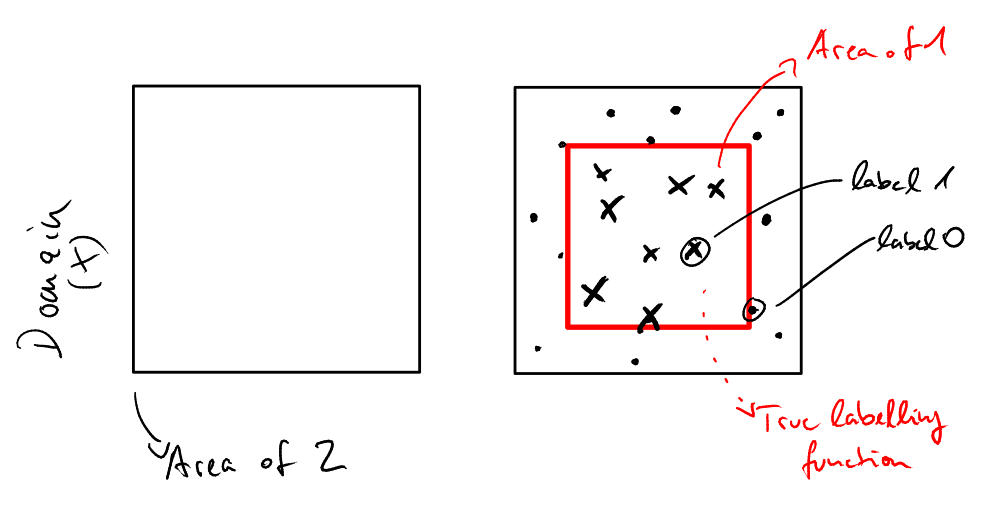
\includegraphics[width=0.7\linewidth]{sketch_1}
	\caption{Problematic Case 1}
	\label{fig:sketch1}
\end{figure}

\begin{itemize}
	\item say the distribution on X is uniform
	\item say we have an ERM algorithm that returns $h_S$ such that 
	\begin{align*}
			 h_s(x) &= \begin{cases}
			y_i , &  \text{if } \exists \ i \in [m]: x_i = x  \\
			0 , &  \text{else} 
		\end{cases} && \text{(a lookup table)} 
	\end{align*}
\end{itemize}
Obviously $h_S$ is correct on our training set $\implies$ \colorbox{Apricot}{$L_S(h_S) = 0 \text{ !}$}
But on unseen instances from $\mathcal{D} (X \sim \mathcal{D})$, $h_S$ is only correct 50\% of the time (due to the ratio of the areas of the black and red squares in the sketch): $\implies $ \colorbox{Apricot}{$L_{\mathcal{D},f}(h_S) = \frac{1}{2} \text{ !}$}
This is called \textbf{overfitting}.

\paragraph{Hypothesis class (H):} We restrict searching for h to H, i.e., a class of functions from X to Y, and write:
$$
\text{ERM} = \text{ERM}_{H} (\mathcal{S}) \in \text{argmin}_{h \in H} L_{\mathcal{S}}(h)
$$
\underline{Remark:} In our previous example, we did not do this and allowed to memorize the training data!

\section{ERM over finite hypothesis classes $(\big|H\big| < \infty)$}
\underline{Assumption (realizability):} $ \exists \ h^*\in H \text{ with } L_{\mathcal{D},f}(h^*) = 0$\\
\newline
Now, any ERM hypothesis $h_\mathcal{S}$ will attain 0 empirical error ($L_\mathcal{S}(h_\mathcal{S}) = 0$), as it computes with $h^*$ (which obviously has 0 empirical error).\\
\newline
Hence, $L_{\mathcal{D},f}(h_\mathcal{S}) > \varepsilon$ can only happen if we select a hypothesis with $L_\mathcal{S}(h_\mathcal{S}) = 0$ but $L_{\mathcal{D},f}(h_\mathcal{S}) > \varepsilon$ (trivially).\\
 We can write
\begin{align*}
	H_\text{\textcolor{red}{bad}} &= \{h \in H: L_{D,f}(h)>\varepsilon\} && \text{ set of \textcolor{red}{bad} hypotheses}\\
\end{align*}

Also, we define
\begin{align*}
	M &= \{\mathcal{S}|_x : \exists h \in \underbrace{H_{\mathrm{\textcolor{red}{bad}}}}_{
		\mathclap{  \text{ those are the ones with generalization error $\geq \varepsilon$ } }
		}, L_\mathcal{S}(h) = 0  \}\\
\end{align*}

We observe:
\begin{align*}
	\big\{\mathcal{S}|_x : L_{\mathcal{D},f}(\underbrace{h_\mathcal{S}}_{\mathclap{\text{Empirical risk minimizer}}}) \geq \varepsilon\big\} &\subseteq \big\{\mathcal{S}|_x : \exists \ h \in H_{\mathrm{\textcolor{red}{bad}}}, L_\mathcal{S}(h) = 0 \big\}= M\\
	 \implies M &= \bigcup_{h \in H_{\mathrm{\textcolor{red}{bad}}}}\{\mathcal{S}|_x: L_{\mathcal{S}}(h) = 0\}
\end{align*}
We get (upon measuring with $\mathcal{D}$):
\begin{align*}
\mathcal{D}^m \big( \{\mathcal{S}|_x : L_{\mathcal{D},f}(h_\mathcal{S}) \geq \varepsilon\}\big) &\leq \mathcal{D}^m\left( \bigcup_{h \in H_{\mathrm{\textcolor{red}{bad}}}}\{\mathcal{S}|_x : L_{\mathcal{S}}(h) = 0\} \right)\\
&\leq \sum_{h \in H_{\mathrm{\textcolor{red}{bad}}}} \mathcal{D}^m \big(\{\mathcal{S}|_x : L_{\mathcal{S}}(h) = 0\}\big) && \text{(due to $\sigma$-sub-additivity \textcolor{red}{"Union Bound"})}
\end{align*}
\underline{Let's fix some $h \in H_{\mathrm{\textcolor{red}{bad}}}$:}
\begin{align*}
	D^m \big(\{\mathcal{S}|_x : L_{\mathcal{S}}(h) = 0\}\big) 
		&= \mathcal{D}^m \left(\left\{\mathcal{S}|_x : \forall i \in [m]: h(x_i) = f(x_i)\right\}\right)\\
		&= \prod_{i = 1}^{m} \mathcal{D} \left(\{x_i: h(x_i) = f(x_i)\} \right) 	&& \text{(due to iid assumption)}\\
		&= \prod_{i=1}^{m} (1 - L_{\mathcal{D},f}(h))\\
		&\leq \prod_{i=1}^{m} (1-\varepsilon)		&& \text{(as $h \in H_{\mathrm{\textcolor{red}{bad}}}$)}\\
		&= (1-\varepsilon)^m \\
		&\leq e^{-\varepsilon m}
\end{align*}
So, to conclude:
\begin{align*}
	D^m \big(\{\mathcal{S}|_x : L_{\mathcal{D},f}(h_S) \geq \varepsilon\}\big) &\leq \sum_{h \in H_{\mathrm{\textcolor{red}{bad}}}} e^{-\varepsilon m} \\ 
	&= |H_{\mathrm{\textcolor{red}{bad}}}| \cdot e^{-\varepsilon m} \\
	&\leq |H| \cdot e^{-\varepsilon m}
\end{align*}

This is a probabilistic guarantee that tells us how the generalization error scales with the sample size. If we let 

	$$ |H| \cdot e^{-\varepsilon m} <\delta \in (0,1)$$ 

and solve for $m$, we get 

	$$ m > \frac{1}{ \underbrace{ \varepsilon}_{\mathclap{\text{error}}}} \cdot \log \Big(\frac{|H|} {\underbrace{\delta}_{\mathclap{\text{confidence}} }}\Big)$$
	
\begin{corollary}
	Let $|H| < \infty$ and $\varepsilon, \delta \in (0,1)$. Further, let $m$ be an integer (the sample size) such that $\color{red} m>\frac{1}{\varepsilon} \cdot \log\big(\frac{|H|}{\delta}\big)$. Then, for each labeling function $f: \mathcal{X} \to \mathcal{Y}$ and any distribution $\mathcal{D}$ over domain $\mathcal{X}$ (for which realizability holds), we have that with probability of at least $1-f$ over the choice of $S|_x$ (of size m) it holds that every ERM hypothesis $h_s$ satisfies the following:
	$$ L_{\mathcal{D},f}(h_s) \leq \varepsilon $$
\end{corollary}

\textcolor{red}{\paragraph{Interpretation:} For sufficiently large $m, ERM_H$ returns $h_S$ (i.e., a hypothesis) that is \textbf{P}ROBABLY \textbf{A}PPROXIMATELY \textbf{C}ORRECT (PAC).}\\

\section{PAC learnability}

\begin{boxeddef}[PAC learnability]
	A hypothesis class $H$ is \textcolor{red}{\textbf{PAC learnable}}, if there exists a function $m_H: (0,1)^2 \to \mathbb{N}$ and a learning algorithm $\mathcal{A}$ with the following properties:
	\begin{enumerate}
		\item for every $\varepsilon, \delta \in (0,1)$, and
		\item every distribution $\mathcal{D}$ over domain $\mathcal{X}$, and
		\item every labelling function $f: \mathcal{X} \to \{0, 1\}$, if
		\item realizability holds (w.r.t. to $\mathcal{D}, H, f$) then
	\end{enumerate}
	running $\mathcal{A}$ on $m \geq m_H(\varepsilon, \delta)$ \textit{iid.} instances drawn from $\mathcal{D}$ and labelled by $f$, returns a hypothesis $h$ such that with probability of at least $1-\delta$ (over choice of S) 
	$$ L_{\mathcal{D}, f} \leq \varepsilon $$
\end{boxeddef}

\begin{boxedsubdef}[Sample complexity]
	$m_H: \{0,1\} \to \mathbb{N}$ is called the \textcolor{red}{sample complexity} function. In particular, $m_H$ returns the smallest integer such that the requirements for PAC-learnability are satisfied.
\end{boxedsubdef}
We have already seen that \textcolor{red}{finite hypothesis classes} ($|H| < \infty$) \textcolor{red}{are PAC learnable} with 
$$ m_H(\varepsilon, \delta) \leq \bigg\lceil\frac{1}{\varepsilon} \cdot log \bigg( \frac{|H|}{\delta}\bigg) \bigg\rceil $$
\newpage

We will now move to a more general setting.
\begin{enumerate}[label*=\protect\fbox{\arabic{enumi}}]
	\item We will first release the realizability assumption (In this setting, the best we can hope for are guarantees relative to the "best" possible hypothesis in the class: $\min_{h \in H}{L_{\mathcal{D}, f}(h)}$)
\end{enumerate}
	\begin{boxeddef}[Höffding inequality]
	Let $X_1, ..., X_m$ be \textit{iid} random variables taking values in $[a_i, b_i]$ for $i \in [m]$. Then, it holds that
	 \begin{align*}
	 	\mathbb{P}\left[S_m - \mathbb{E}[S_m] > \varepsilon\right] 
	 		&\leq e^{\left(\frac{-2 \varepsilon^2}{\sum_{i} (b_i - a_i)^2}\right)} 
	 			&& \hspace{0.4cm} S_m = \sum_{i = 1}^{m} X_i, \text{ and}\\
	 	\mathbb{P}\left[S_m - \mathbb{E}[S_m] < -\varepsilon\right] 
	 		&\leq e^{\left(\frac{-2 \varepsilon^2}{\sum_{i} (b_i - a_i)^2}\right)}\\
	 	\intertext{\underline{Also:}}\\
	 	\mathbb{P}\bigg[\big|S_m - \mathbb{E}[S_m]\big| > \varepsilon\bigg] 
	 		&\leq 2 \cdot e^{\frac{-2 \varepsilon^2}{\sum_{i} (b_i - a_i)^2}}\\
	 	\text{(As we have $|a| \geq b \Leftrightarrow a \leq -b \text{ \underline{OR} } a \geq b$)}
 	\end{align*}


\end{boxeddef}
Another useful form of this inequality is:
$$ 
	\mathbb{P} \left[\left| \frac{1}{m} \cdot \sum_{i = 1}^{m} X_i - \mu \right| > \varepsilon\right] \leq 2 e^{\frac{-2 \varepsilon^2 m}{b-a}} 
$$
with $\mu = \mathbb{E}[X_i]$ and $\mathbb{P}[a \leq X_i \leq b] = 1$ for all $i \in [m]$.\\
 As a consequence, we can say the following: fix $\varepsilon>0$; then for any \colorbox{Apricot}{\underline{single} $h: \mathcal{X} \to \mathcal{Y}$}, we have 
$$ 
	\mathbb{P}_{S|_x \sim \mathcal{D}^m}\left[\left|L_{s}(h) - L_{\mathcal{D}, f}\right| > \varepsilon\right] \leq 2 e^{-2\varepsilon^2 m} \hspace{1cm} (a = 0, \ b = 1)
$$

If we would set $\delta = 2^{-2 \varepsilon^2 m}$, and solve for $\varepsilon$, we would get
\begin{align*}
\varepsilon &= \sqrt{\frac{log\big(\frac{2}{\delta}\big)}{2m}}\\
\implies L_{\mathcal{D},f}(h) &\leq L_{s}(h) + \sqrt{\frac{log\big(\frac{2}{\delta}\big)}{2m}}\\
\text{\textcolor{red}{(holds with probabilty of }} & \text{\textcolor{red}{at least $1-\delta$ over choice of S)}}
\end{align*}

\begin{remark}
	This result holds for a \underline{single} h. However, we can easily get a bound that holds \underline{uniformly} for all $h \in H, |H| < \infty$
\end{remark}

$$ \mathbb{P}_{S|_x \sim \mathcal{D}^m} \bigg[\exists h \in H: \big|L_{s}(H) - L_{\mathcal{D}, f}(h) \big| > \varepsilon \bigg] \leq \sum_{h \in H} 2\cdot e^{-2 \varepsilon^2 m} \leq 2 \big|H\big| \cdot e^{-2 \varepsilon^2 m} $$ 
We will see that we did need realizability for that!

\begin{enumerate}
	\item[\protect\fbox{2}] Next, we release our requirement of a "true" labelling function $f$. We do this by letting $\mathcal{D}$ be a distribution over $\mathcal{X} \times \mathcal{Y} = \mathcal{Z}$. We need to adjust our definitions of empirical error and generalization error:
	\begin{eqnarray}
		L_{\mathcal{D}}(h) = 
			\mathbb{P}_{(x, y) \sim \mathcal{D}} \left[h(x) \neq y\right] = 
			\mathcal{D}\big( \{(x,y) \in \mathcal{X} \times \mathcal{Y}: h(x) \neq y\} \big)\\
		L_{\mathcal{S}}(h) = \frac{1}{m} \cdot \big| \{ i \in [m]: h(x_i) \neq y_i \} \big|	
	\end{eqnarray}
\end{enumerate}

Both \protect\fbox{1} and \protect\fbox{2} lead to:
\section{Agnostic PAC learnability}
\begin{boxeddef}[Agnostic PAC learnability]
	A hypothesis class $H$ is \textcolor{red}{agnostic PAC learnable}, if there exists a function $m_H: (0,1)^2 \to \mathbb{N}$ and a learning algorithm $\mathcal{A}$ with the following properties:
	\begin{enumerate}
		\item for every $\varepsilon, \delta \in (0,1)$ and
		\item every distribution $\mathcal{D}$ over domain $\mathcal{X} \times \mathcal{Y}$
	\end{enumerate}
	running $\mathcal{A}$ on $m \geq m_H(\varepsilon, \delta)$ \textit{iid.} instances drawn from $\mathcal{D}$, returns a hypothesis $h$ such that with probability of at least $1-\delta$ (over choice of S) 
	\textcolor{red}{$$ 
		L_{\mathcal{D}}(h) \leq \min_{h' \in H} L_{\mathcal{D}}(h') + \varepsilon
		$$}
\end{boxeddef}
Implicit assumption: the best possible thing from the hypothesis class is at least okay. If it is large, then the min is large, and consequently the threshold is bad!\\
To show that \textit{finite classes are agnostic PAC learnable}, we will use the Höffding inequality.

\subsection{General loss functions}
	$$ l: H \times ( \underbrace{\mathcal{X} \times \mathcal{Y}}_{\mathclap{\mathcal{Z}}}) \to \mathbb{R}_+ $$
Example: \textcolor{red}{0-1 loss}\\
$$ l^{0-1}\left( h, \left(x,y\right) \right) = \begin{cases}
	1, &  \text{if } h(x) \neq y  \\
	0, &  \text{else} 
\end{cases}$$

\textcolor{red}{square loss:}
$$
l^{sq}(h, \underbrace{\left(x,y\right)}_{\text{e.g.} \in \mathbb{R}}) =  \left(y-h(x)\right)^2 \hspace{1.5cm}\text{\textit{e.g. in regression problems}}
$$
In case of general loss functions, we adjust our definitions of $L_\mathcal{D}$ and $L_\mathcal{S}$ as follows:
$$ 
L_\mathcal{D}(h) =  \mathbb{E}_z[l(h, z)], \ \  L_\mathcal{S}(h) = \frac{1}{m} \cdot \sum_{i = 1}^{m} l(h, z_i)
$$

\begin{remark}
	\begin{align*}
		\mathbb{E}_z\left[l^{0-1}(h,z)\right] 
			&= 0 \cdot \mathbb{P}_z[h(x) = y] + 1 \cdot \mathbb{P}_z[h(x) \neq y]\\
			& = \mathbb{P}_z[h(x) \neq y]
	\end{align*}
\end{remark}

\section{Uniform convergence}
\begin{boxeddef}[$\varepsilon$-representative sample]
	A sample S is called \textcolor{red}{$\varepsilon$-representative sample} wrt. $\mathcal{Z} (= \mathcal{X}\times\mathcal{Y})$, loss function $l$ and distribution $\mathcal{D}$, if
	$$
	\forall h \in H: \left|L_S(h) - L_\mathcal{D}(h)\right| \leq \varepsilon
	$$
\end{boxeddef}

\begin{lemma}
	Assume that S is $\frac{\varepsilon}{2}$-representative w.r.t. $\mathcal{Z}, H, l$ and $\mathcal{D}$. Then, any hypothesis \textcolor{red}{$h_S$} returned by $ERM_H(S) \in argmin_{h' \in H}(L_\mathcal{S}(h'))$ satisfies
	$$
	L_D(\text{\textcolor{red}{$h_S$}}) \leq \min_{h \in H} L_D(h) + \varepsilon
	$$
\end{lemma}

\begin{proof}
For any $h \in H$:
\begin{align*}
	L_\mathcal{D}(h_s) 
		&\leq L_S(h_S) + \frac{\varepsilon}{2}  
			&&\text{(by def. $\varepsilon$-representativeness)}\\
		&\leq L_S(h) + \frac{\varepsilon}{2} 
			&&\text{(as $h_S$ is ERM-hyp.)}\\
		&\leq L_\mathcal{D}(h) + \frac{\varepsilon}{2} + \frac{\varepsilon}{2}
			&& \text{(by def. $\varepsilon$-representativeness)}\\
		&\leq  L_\mathcal{D}(h) + \varepsilon
\end{align*}
As this inequality chain holds for any $h \in H$, we conclude that $$L_\mathcal{D}(h_S) \leq \min_{h \in H} L_\mathcal{D}(h) + \varepsilon$$
\end{proof}
This leads us to the definition of uniform convergence:
\begin{boxeddef}[Uniform convergence]
	A hypothesis class $H$ has the \textcolor{red}{uniform convergence (UC)} property (wrt. $\mathcal{Z}$ and loss function $l$) if there exists\\
	 $m_H^{UC}: (0,1)^2 \rightarrow \mathbb{N}$ such that for every $\varepsilon, \delta \in (0,1)$ and every distribution $\mathcal{D}$ over $\mathcal{Z}$, if $\mathcal{S}$ is an iid sample of size $m \geq m_H^{UC}(\varepsilon, \delta)$ from $\mathcal{D}$, then with probability of at least $1-\delta$ (over the choice of $\mathcal{S}$), $\mathcal{S}$ is $\varepsilon$-representative
\end{boxeddef}

\begin{corollary}
	If $H$ has the UC property with $m_H^{UC}$, then $H$ is agnostic PAC learnable with 
	$$ m_H(\varepsilon, \delta) \leq m_H^{UC}(\frac{\varepsilon}{2}, \delta)$$
	Moreover, ERM is a successful APAC learner for H!
\end{corollary}

\begin{claim}
	Finite $H$ ($|H|< \infty$) are agnostic PAC learnable.
	Given fixed $\varepsilon, \delta \in (0,1)$, we want to show that
	\begin{align*}
		D^{m}\Big(\big\{\mathcal{S}: \forall h \in H: \left|L_S(h) - L_D(h) \right| 
			&\leq \varepsilon\big\}\Big) \geq 1-\delta\\
		\intertext{Equivalently,}\\
		D^{m}\Big( \underbrace{ \big\{ \mathcal{S}: \exists h\in H: \big|L_\mathcal{S}(h)-L_\mathcal{D}(h)\big|\textcolor{red}{> }\varepsilon \big\}}_{\mathclap{\bigcup_{h \in H} \left\{\mathcal{S}: |L_\mathcal{S}(h)-L_\mathcal{D}(h) | > \varepsilon \right\}}} \Big)  
			&< \delta\\
		\intertext{We bound}\\
		\mathcal{D}^m \left( \bigcup_{h \in H} \left\{\mathcal{S}: |L_\mathcal{S}(h)-L_\mathcal{D}(h) | > \varepsilon \right\} \right) 
			&\underbrace{\leq}_{\smash{\text{by union bound }}} \sum_{h \in H} D^m\bigg( \big\{ \mathcal{S}: |L_\mathcal{S}(h)-L_\mathcal{D}(h) | > \varepsilon \big\}  \bigg)
	\end{align*}
\end{claim}

\begin{proof} Lets fix $ l = l^{0-1}$. As we know that $L_D(h) = \mathbb{E}(l(H, z))$ and $L_s(h) = \frac{1}{m} \sum_{i = 1}^{m} l(h, z_i)$, we can use Höffding's inequality (with $b = 1, a=0$): 
	$$D^{m}(\{ S: \exists h \in H: |L_S(h) - L_D(h)| > \varepsilon\}) \leq \sum_{h \in H} 2 \cdot e^{-2 \varepsilon^2 m} = 2 \cdot |H| \cdot  e^{-2 \varepsilon^2 m}$$
Let $e^{-2 \varepsilon^2 m}$ be smaller than $\delta$, i.e.,
	\begin{align*}
		2 |H| \cdot  e^{-2 \varepsilon^2 m} < \delta &\iff m > \log\left( \frac{2 \cdot |H|}{\delta}\right)\cdot \frac{1}{2 \varepsilon^2}\\
		\intertext{This gives us the \underline{sample complexity function} $m_{H}^{UC}$ for uniform convergence. In other words, for l: $H \times \mathcal{Z} \rightarrow [0,1]$, we have shown}\\
		m_H^{UC}(\varepsilon, \delta) &\leq \bigg\lceil \log \left(\frac{2 \cdot|H|}{\delta} \cdot \frac{1}{2 \varepsilon^2}\right) \bigg\rceil\\
		\intertext{and by our earlier corollary we get for the sample complexity function $m_{H}$ for \underline{agnostic PAC learnability}}\\
		m_H(\varepsilon, \delta) \leq m_H^{UC}\left(\frac{\varepsilon}{2}, \delta\right) &\leq \left\lceil \frac{2 \cdot \log\left(\frac{2\cdot |H|}{\delta}\right)}{\varepsilon^2} \right\rceil
	\end{align*}
This establishes the claim.
\newpage
\end{proof}

The first case that causes problems with this definition:
\begin{figure}[H]
	\centering
	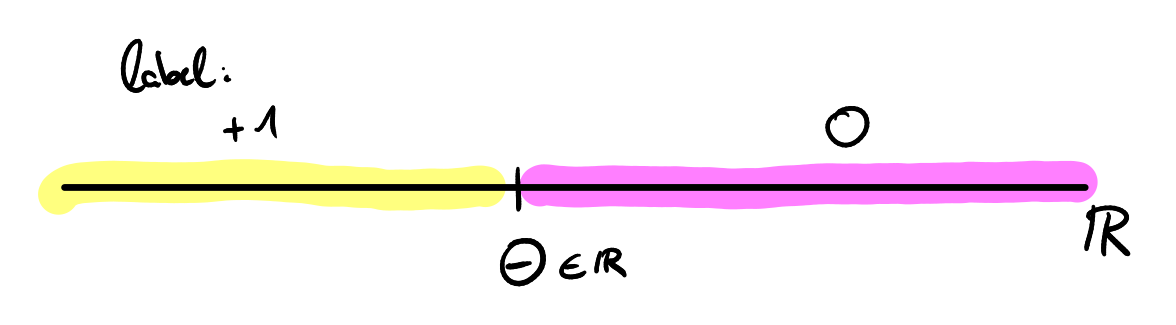
\includegraphics[width=0.7\linewidth]{sketch_2}
	\caption{Problematic Case 2}
	\label{fig:sketch2}
\end{figure}

\paragraph{Question:} Is there a "universal" learner?, i.e. a learner \textit{without any prior knowledge} (w.r.t. $H, \mathcal{D, ...}$) of a task (\textcolor{red}{specified by $\mathcal{D}$}), but can be challenged by any task (and achieves low $L_\mathcal{D}\left(A\left(s\right)\right)$). 

\section{No-Free-Lunch Theorem}
\begin{theorem}[No-Free-Lunch]	
Let A be a learning algorithm for the task of binary classification with respect to 0-1 loss over a domain $\mathcal{X}$. Also, let $m$ be any number smaller than $|\mathcal{X}|\textfractionsolidus2$, representing the training set size. Then, there exists a distribution $\mathcal{D}$ over $\mathcal{X} \times \left\{0, 1\right\}$ such that 
\begin{enumerate}
	\item $\exists f: \mathcal{X} \to \left\{0,1\right\} \text{with } L_\mathcal{D}(f) = 0$
	 \item with probability of at least $\frac{1}{7}$ over the choice of $S \sim \mathcal{D}^m$, we have\\
	 $$ L_\mathcal{D}\big(A(s)\big) \geq \frac{1}{8}.$$
\end{enumerate}
2. means that the learner fails on that task; 1. means that the task can be successfully learned by another learner (e.g. ERM$_{\mathcal{H}}$ for $H = \left\{f\right\}$).
\end{theorem}

\begin{proof}
	Let $C \subset \mathcal{X}$ be of size \textcolor{red}{$2m$}, $|C| = 2m$. The number of possible labellings of C is  $T = 2^{2m}$ (as we have 2m labels with 2 possibilities each). Lets denote the functions which realize these T labellings as 
	$$ f_1 , ..., f_T $$
	For \underline{each $f_i$}, we define the following:
	\begin{align*}
		\underbrace{\mathcal{D}_{\textcolor{red}{i}}\big(\left\{(x,y)\right\}\big)}_{\text{defines a task}} = \begin{cases}
				\frac{1}{|C|} , &  \text{if $y = f_{\textcolor{red}{i}}(x)$}\\
				0 , &   \text{else} 
		\end{cases}
	\end{align*}
	Hence, by construction 
	$$
		L_{\mathcal{D}_{\textcolor{red}{i}}}(f_{\textcolor{red}{i}}) = 0
	$$
	With that in mind, we will show that for every learning algorithm A that receives m samples from $\mathcal{X} \times \left\{0,1\right\}$ , there exists a function $f: \mathcal{X} \to \left\{0,1\right\}$ and a distribution $\mathcal{D}$ over $\mathcal{X} \times \left\{0,1\right\}$ such that

		\begin{enumerate}

			\item $L_\mathcal{D}(f) = 0$, and
			\item $\mathbb{E}_{S \sim \mathcal{D}^m}\big[L_\mathcal{D}(A(s))\big] \geq \frac{1}{4}$ \hspace{1cm} \textbf{(*)}
		\end{enumerate}	
	In particular, we show that for every learning algorithm A receiving m samples from $C \times \left\{0,1\right\}$ and returning a function $A(S): X \to \left\{0,1\right\}$, we have
	
	$$
		\max_{i \in [T]} \mathbb{E}_{S \sim D^{m}_{\textcolor{red}{i}}}\bigg[L_{\mathcal{D}_{\textcolor{red}{i}}}\big(A(s)\big)\bigg] \geq \frac{1}{4} \hspace{1cm} \text{\textbf{(**)}}
	$$
	\begin{remark}
		\textbf{(*)} suffices for $L_D(A(s)) \geq \frac{1}{8}$ with probability of at least $\frac{1}{7}$ over the choice of $S \sim D^m$ (see PS exercise!)
	\end{remark}
	
	\paragraph{Lets show that (**) holds:} We know that there are \textcolor{red}{$(2m)^m = k$} possible training sequences of size m (remember $|C| = 2m$) from $C$. Lets call them
	$$ S_1, ..., S_k $$
	Also, lets call $S_{\textcolor{orange}{j}}^{\textcolor{red}{i}}$ the sequence $S_{\textcolor{orange}{j}}$ labelled by $f_{\textcolor{red}{i}}$, i.e.,
	$$
	 S_{\textcolor{orange}{j}}^{\textcolor{red}{i}} = \bigg( \big(x_1, f_i(x_i)\big), ..., \big(x_m, f_i(x_m)\big)\bigg)
	$$ 
	$$
		\text{with } S_{\textcolor{orange}{j}} = (x_1, ..., x_m)
	$$
	Now, in case the distribution is $\mathcal{D}_i$, then $S_1^{\textcolor{red}{i}}, ..., S_k^{\textcolor{red}{i}}$ are the possible training sequences that A can receive. Note that, by construction of the $\mathcal{D}_i$, \underline{all} these training sequences have equal probability of being drawn/sampled.
	$$
		\Rightarrow\mathbb{E}_{S \sim D^{m}_{\textcolor{red}{i}}}\bigg[L_{\mathcal{D}_{\textcolor{red}{i}}}\big(A(s)\big)\bigg] = \underbrace{\frac{1}{k}}_{\mathclap{  \text{no. of possible training sequences of size m}}} \cdot \sum_{j = i}^{k} L_{\mathcal{D}_i}(A(S_{j}^{i})) \hspace{1cm} \text{\textbf{(***)}}
	$$ 
	$\Big($Lets remember that we want to show
	$
		\max_{i \in [T]} \mathbb{E}_{S \sim D^{m}_{\textcolor{red}{i}}}\big[L_{\mathcal{D}_{\textcolor{red}{i}}}\big(A(s)\big)\big] \geq \frac{1}{4}
	$ $\Big)$
	\begin{align*}
		\max_{i \in [T]} \mathbb{E}_{S \sim D^{m}_{\textcolor{red}{i}}}\bigg[L_{\mathcal{D}_{\textcolor{red}{i}}}\big(A(s)\big)\bigg] 
			&= \max_{i \in [T]} \frac{1}{k} \cdot \sum_{j = i}^{k} L_{\mathcal{D}_i}(A(S_{j}^{i})) 
				&& \text{by \textbf{(***)}} \\
			&\geq \frac{1}{T} \cdot \sum_{i=1}^{T} \frac{1}{k} \sum_{j = i}^{k} L_{\mathcal{D}_i}(A(S_j^i))
				&& \text{(as $\max \geq$ avg)} \\
			&= \frac{1}{k} \cdot \sum_{j=1}^{k} \frac{1}{T} \sum_{i = 1}^{T} L_{\mathcal{D}_i}(A(S_j^i))\\
			&\leq \min_{j \in [k]} \frac{1}{T} \cdot \sum_{i = 1}^{T} L_{\mathcal{D}_i}(A(S_j^i))
	\end{align*}
	
	\paragraph{Lets fix some $j \in [k]$:}
	$$(S_j = (x_1, ..., x_m))$$
	As $S_j$ is of size m, but C is of size $2m$, there are instances from C which we have not seen. Lets call them 
	$$ V_1, ..., V_p$$
	We also know that \textcolor{red}{$p \geq m$}.\\
	
	For every $h: C \to \left\{0,1\right\}$ and every i, it holds that 
	\begin{align*}
		L_{\mathcal{D}_i}(h) &= \frac{1}{2m} \cdot \sum_{x \in C} \mathbbm{1}_{h(x) \neq f_i(x)}\\
		&\geq \frac{1}{2m} \cdot \sum_{r = 1}^{p} \mathbbm{1}_{h(v_r) \neq f_i(v_r)}\\
		&\underbrace{\geq}_{\mathclap{\text{as } p \geq m}} \frac{1}{2p} \sum_{r = 1}^{p}  \mathbbm{1}_{h(v_r) \neq f_i(v_r)} && \text{\textbf{(****)}}
	\end{align*}
	
	Combining results gives 
\begin{align*}
		\frac{1}{T} \cdot \sum_{i = 1}^{T} L_{\mathcal{D}_i}(A(S_j^i)) &\geq \frac{1}{T} \cdot \sum_{i = 1}^{T} \frac{1}{2p} \sum_{r = 1}^{p} \mathbbm{1}_{A(S_j^i)(v_r) \neq f_i(v_r)}\\
		\intertext{(A run on $S_j^i$ gives some $h: C \to \left\{0,1\right\}$ and we know that (****) holds for every $h: C \to \{ 0,1 \}$)}\\
		&= \frac{1}{2} \cdot \frac{1}{p} \sum_{r = 1}^{p}\frac{1}{T} \sum_{i = 1}^{T} \mathbbm{1}_{A(S_j^i)(v_r) \neq f_i(v_r)}\\
		&\geq \frac{1}{2} \min_{r \in [p]} \frac{1}{T} \sum_{i = 1}^{T} \mathbbm{1}_{A(S_j^i)(v_r) \neq f_i(v_r)} 
			&& \text{(as avg $\geq$ min)}
\end{align*}
\paragraph{Lets fix some $r \in [p]$:} Remember that we have $f_1, ..., f_T$ (for $T = 2^{2m}$ labelings).\\
\underline{Example:} say $m = 1, |C| = 2$
\begin{table}[H]
	\begin{tabular}{lll|l}
		&  & $c_1$ & $v_1$ \\ \cline{3-4} 
		\textcolor{purple}{$f_1$} &  & 0     & 0     \\
		\textcolor{purple}{$f_2$} &  & 0     & 1     \\
		\textcolor{purple}{$f_3$} &  & 1     & 0     \\
		\textcolor{purple}{$f_4$} &  & 1     & 1    
	\end{tabular}
\end{table}

Partition into 2 pairs (\textcolor{purple}{$f_1, f_2$}) and (\textcolor{purple}{$f_3, f_4$}), where (\textcolor{purple}{$f_1, f_2$}) only differ by $v_1$ \underline{and} (\textcolor{purple}{$f_3, f_4$}) only differ by $v_1$.\\
In general, we can partition into \textcolor{red}{T\textfractionsolidus 2} disjoint pairs of functions ($f_i$'s). For every pair $(f_i, f_i')$ we have that for every $c \in C$
$$
	f_i(C) \neq f_i'(C) \text{\textbf{ if and only if }} c = v_r
$$
For such a pair, we have $S_j^{i} = S_{j}^{i'}$. Consequently, we have 
$$
	\mathbbm{1}_{A(S_j^i)(v_r)) \neq f_i(v_r)} + \mathbbm{1}_{A(S_j^{i'})(v_r)) \neq f_i(v_r)} = \textcolor{red}{1}
$$
Rememebering that we had $\frac{1}{T} \sum_{i=1}^{T} \mathbbm{1}_{A(S_j^i)(v_r)) \neq f_i(v_r)}$ and now re-writing the sum as a  sum over all disjoint pairs, we get in combination with \textbf{(****)}
$$
 \frac{1}{\cancel{T}} \cdot \frac{\cancel{T}}{2} = \frac{1}{2}
$$
\textbf{Overall:}
\begin{align*}
	\max_{i \in [T]} \ \mathbb{E}_{\mathcal{S} \sim \mathcal{D}_i^m}[L_{\mathcal{D}_i}(A(S))]  &\geq \frac{1}{2} \cdot  \min_{r \in [p]} \underbrace{\frac{1}{T} \sum_{i=1}^{T} \mathbbm{1}_{A(S_j^i(v_r)) \neq f_i(v_r)}}_{\mathclap{ = \frac{1}{2}}}\\
	&= \frac{1}{2} \cdot \frac{1}{2} = \frac{1}{4}
\end{align*}

Our earlier steps of fixing indices in the min-operations are irrelevant as we get a constant lower bound!
\end{proof}
\begin{corollary}
	 Let $\mathcal{X}$ be an infinitely large domain and let $H$ be the set of \underline{all} functions $\mathcal{X} \to \{0,1\}$. Then, H is \underline{not} PAC-learnable.
\end{corollary}
\begin{proof} Assume towards contradiction that H is PAC-learnable. Then, it would have a sample size function. Then, we would just have to make the $\varepsilon$ small enough to violate the NFL-theorem.
\end{proof}

\section{Vapnik-Chervonenkis Dimension (VC Dimension)}
If we review the proof of the NFL theorem, it seems intuitive to study how a hypothesis class H behaves on C.
\begin{boxeddef}
	Let H be a class of functions from $X \to \{0,1\}$ and let $C \subset X, C = \{c_1, ..., c_m \}$. We define 
	$$ H_C = \{ (h(c_1), ..., h(c_m)): h \in H\} $$
	as the restriction of H to C.
\end{boxeddef}

\paragraph{Example:}
\begin{enumerate}
	\item $C = \{c_1\}, c_1 \in \mathbb{R}$; lets look at the class H of thresholds
	\begin{figure}[H]
		\centering
		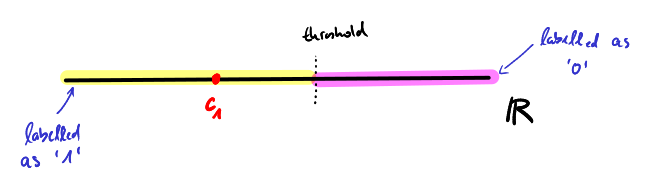
\includegraphics[width=0.9\linewidth]{sketch_3}
		\label{fig:sketch3}
	\end{figure}
	$ H_C = \{(1), (0)\}, |H_C| = 2^1 = 2$
	\item $C = \{c_1, c_2\}$
		\begin{figure}[H]
			\centering
			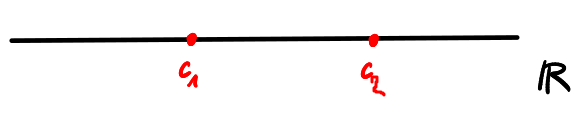
\includegraphics[width=0.7\linewidth]{sketch_3-2}
			\label{fig:sketch3-2}
		\end{figure}
		$ H_C = \{(0,0), (0,1), (1,1)\}, \ |H_C| = 3 $ (the labelling $(1,0)$ is not possible, as the threshold would need to be $\leq c_1 \land \geq c_2$!)
\end{enumerate}

\begin{boxedsubdef}
	H \textcolor{red}{shatters} a finite set C of size m, if $|H_C| = 2^m$
\end{boxedsubdef}

\paragraph{Example:}
The class of thresholds on $\mathbb{R}$ is PAC-learnable.
\begin{align*}
	H^{\text{thr}} = \{h_a: a \in \mathbb{R}\}&, h_a: \mathbb{R}\to\{0,1\}\\
	x \mapsto h_a(x) &= \mathbbm{1}_{x<a} = 
	\begin{cases}
		1 , &  \text{if } x<a \\
		0 , &  \text{else} 
	\end{cases}
\end{align*}

\begin{claim} $H^{\text{thr}}$ is PAC learnable with
$$
	m_{H^{\text{thr}}}(\varepsilon, \delta) \leq \left\lceil \log \bigg(\frac{2}{\delta}\bigg) \cdot \frac{1}{\varepsilon}\right\rceil
$$
\end{claim}

\begin{proof} Let $\textcolor{blue}{a_0}$ be such that $\mathcal{D}(\{x\in \mathbb{R}: x \in (\textcolor{blue}{a_0}, \textcolor{red}{a^*})\}) = \varepsilon$; let $\textcolor{blue}{a_1}$ be such that $\mathcal{D}(\{x\in \mathbb{R}: x \in (\textcolor{red}{a^*}, \textcolor{blue}{a_1})\}) = \varepsilon$\\
\underline{The special cases are:}
\begin{itemize}
		\item if $\mathcal{D}(\{x\in \mathbb{R}: x \in (\textcolor{blue}{a_0}, \textcolor{red}{a^*})\}) < \varepsilon$, then set $a_0$ to $-\infty$
		\item if $\mathcal{D}(\{x\in \mathbb{R}: x \in (\textcolor{red}{a^*}, \textcolor{blue}{a_1})\}) < \varepsilon$, then set $a_1$ to $+\infty$
\end{itemize}
	We are given $S = \{(x_1, y_1), ..., (x_m, y_m)\}$. An ERM algorithm would be, e.g., 
	\begin{align*}
		b_0 = \max \{x: (x,1) \in S \}\\
		b_1 = \min \{x: (x,0) \in S \}
	\end{align*}
	Visually,\\
	\begin{figure}[H]
		\centering
		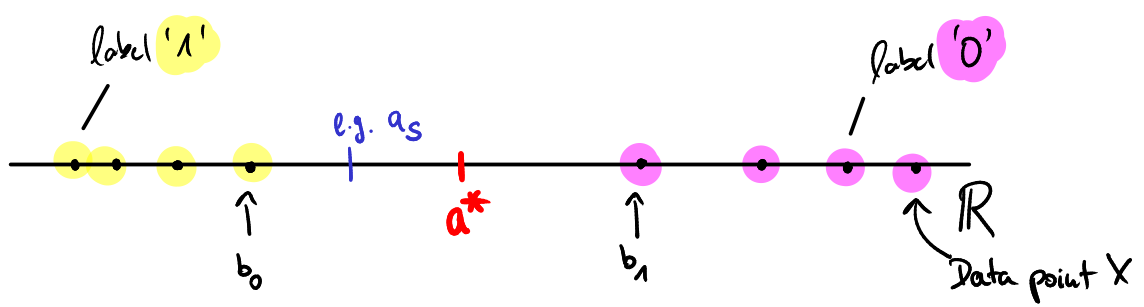
\includegraphics[width=0.9\linewidth]{sketch_5}
		\label{fig:sketch5}
	\end{figure}
	
	so, ERM can choose \underline{any} threshold within $(b_0, b_1)$ (while still having empirical error 0!). Lets denote the threshold of an ERM hypothesis by \textcolor{blue}{\textbf{$a_S$}} and let \textcolor{blue}{\textbf{$h_S$}} be the corresponding hypothesis.\\
	For \textcolor{blue}{\textbf{$h_S$}} (with \textcolor{blue}{\textbf{$a_S$}} as threshold) to have $L_{\mathcal{D}, f}(h_S) \leq \varepsilon$, if suffices that
	\begin{enumerate}
		\item $b_1 \leq a_1$ \underline{AND}
		\item $b_0 \geq a_0$
	\end{enumerate}
	
	\begin{figure}[H]
		\centering
		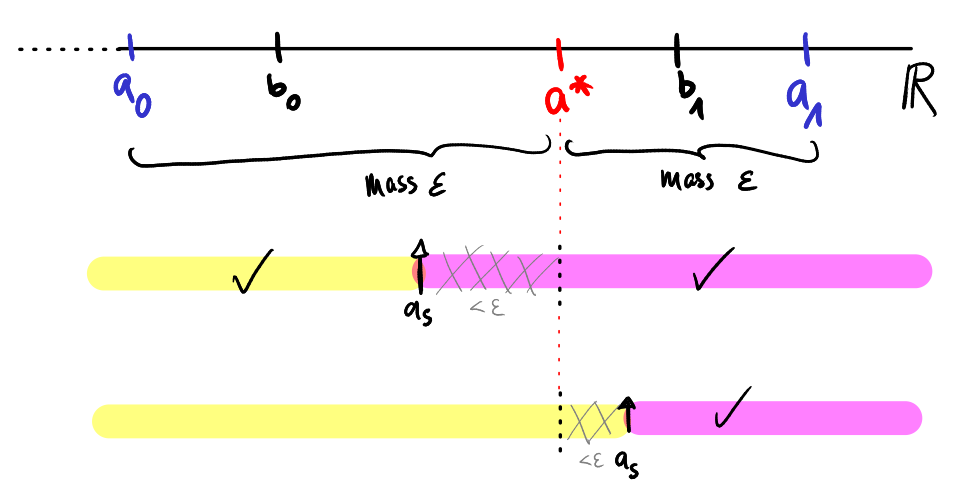
\includegraphics[width=0.7\linewidth]{sketch_6}
		\label{fig:sketch6}
	\end{figure}
	
	In other words, 
	\begin{align*}
		\mathbb{P}\big[L_{D,f}(h_s)>\varepsilon\big] 
			&\leq \mathbb{P}\big[(b_0 < a_0) \lor (b_1 > a_1)\big]\\
			&\leq \mathbb{P}\big[ (b_0<a_0) \big] +\mathbb{P}\big[ (b_1 > a_1) \big]
				&& \text{(union bound)}	
	\end{align*}
	So, when does $b_0 < a_0$ happen? When there is no data point in S that is labelled as 1 s.t. $x \in (a_0, a^*)$ (no data point left of perfect threshold).\\
	We do know that $\mathcal{D}(\{x \in \mathbb{R}: x\in (a_0, a^{*})\}) = \varepsilon$, hence \underline{not seeing} an instance in that interval $(a_0, a^*)$ has probability of $1-\varepsilon$. Not seeing a data point in $m$ \textit{iid} samples thus has probability of \underline{$(1-\varepsilon)^m \leq e^{-\varepsilon m}$}.
	$$
		\implies \mathbb{P}[b_0 < a_0] = (1-\varepsilon)^{m} \leq e^{-\varepsilon m} \text{; same for } \mathbb{P}[b_1>a_1]
	$$
	We get, overall:
	$$
		\mathbb{P}[L_{\mathcal{D}, f}(\ \underbrace{h(s)}_{\mathclap{\text{ERM hyp.}}} \ )>\varepsilon] \leq \underbrace{2 \cdot e^{-\varepsilon m}}_{\mathclap{\text{we want this to be } <\delta}} \ \ \implies m > \log\bigg(\frac{2}{\delta}\bigg) \cdot \frac{1}{\varepsilon}
	$$
\end{proof}

We have seen that "finiteness" of H ($|H| < \infty$) is \underline{sufficient}, but \underline{not necessary} for PAC learnability!

\begin{boxeddef}[VC-Dimension]
	The VC-Dimension of H (a class of functions from $X \to \{0,1\}$) is the \textcolor{red}{maximal} size of a set $C \subset X$ that is shattered by H.
\end{boxeddef}

\begin{theorem}
	Let H be a class of functions from $X \to \{ 0,1 \}$. If H has infinite VC-dimension, then H is \underline{not} PAC-learnable.
\end{theorem}

\begin{proof}
	Without proof, see NFL.
\end{proof}
\begin{boxeddef}[growth function]
	Let H be a class of functions from $X \to \{ 0,1 \}$. The \textcolor{red}{ growth function} of H, $\tau_H: \mathbb{N}_0 \to \mathbb{N}_0$, is defined as 
	\begin{align*}		
		\tau_H (m) = \max_{C \subset X, |C| = m} \big|H_C\big| \hspace{1.5cm} \text{with } \tau_{H}(0)	= 1
	\end{align*}
\end{boxeddef}

\begin{remark} Alternatively, we could define the VC-dim. via $\tau_{H}$:
$$VC(H) = \max\{m\in\mathbb{N}_0, \tau_{H}(m) = 2^{m}\}$$
\end{remark}

\begin{lemma}[Souer, Shelah, Perez; "Souer's Lemma":] Let H be a hypothesis class of functions from $X \to \{ 0,1 \}$ with \textcolor{red}{$VC(H) = d$}. Then
\begin{align*}
	\tau_{H}(m) &= 2^{m} &&\text{ if } m \leq \text{\textcolor{red}{$d$}, but}\\
	\tau_{H}(m) &\leq \left(\frac{e\cdot m}{d}\right)^{d} &&\text{ if } m > \text{\textcolor{red}{$d$}}
\end{align*}
\end{lemma}
\begin{proof}
	Without proof.
\end{proof}

\paragraph{VC-dimension of finite H:} if we take any set C, then its obvious that 
$$ |H_C| \leq |H|$$
Hence, if $|H| < 2^m$, then H cannot shatter C of size m!\\
This implies that 
$$
	VC(H) \leq \log_2(|H|)
$$

\begin{theorem} Let H be a hyp. class of functions from $X \to \{ 0,1 \}$, and $l: H \times \mathcal{X} \times \mathcal{Y} \to [0, c], c > 0$, a loss function. For any distribution $\mathcal{D}$ over $\mathcal{X} \times \mathcal{Y}$ and $\delta \in \{ 0,1 \}$, we have that, with probability of at least $1-\delta$ over the choice of $\mathcal{S} \sim \mathcal{D}^{m}$,:
$$
	\forall h \in H: \big| L_\mathcal{D}(h) - L_\mathcal{S}(H)  \big| \leq c \cdot \sqrt{\frac{8 \cdot \log\left(\tau_{H}(2m) \frac{4}{\delta}\right)}{m}}
$$

\end{theorem}

\textcolor{red}{\begin{theorem}[Fundamental theorem of statistical learning] Let H be a hypothesis class of functions from $X \to \{ 0,1 \}$ and let l be the 0-1 loss. Then, the following statements are equivalent:
\begin{enumerate}
	\item H has the uniform convergence property
	\item Any ERM-algorithm is a successful agnostic PAC-learner for H
	\item H is agnostic PAC-learnable
	\item Any ERM algorithm is a successful PAC-learner for H
	\item H is PAC-learnable
	\item H has finite VC-dimension
\end{enumerate}
\end{theorem}}

\newpage
\part{Linear Predictors}
We define 
$$
	L_d = \{ h_{w,b}: w \in \mathbb{R}^d, b \in \mathbb{R}\} \ \ \ h_{w,b}(x) = \langle w,x \rangle + b
$$
as the class of affine functions. From $L_d$ we get different predictors via composition with some 
\textcolor{red}{$$
	\mathcal{\phi}: \mathbb{R} \to y
$$}
Further, we can use
\begin{align*}
	w' &= (b, w_1, ... , w_d)^T \in \mathbb{R}^{d+1}\\
	x' &= (1, x_1, ... , x_d)^T \in \mathbb{R}^{d+1}
\end{align*}
to write 
$$
	h_{w,b} (x) = \langle w', x' \rangle
$$

If $\mathcal{\phi}: \mathbb{R} \to y$ is \textcolor{red}{$\mathcal{\phi} \equiv \text{sign}$}, we get the so called \textcolor{red}{halfspace predictor}:
$$
	HS_d = \mathcal{\phi} \circ L_d = \{ x \mapsto \text{sign}(h_{w,b}(x)): h_{w,b} \in L_d \}
$$

\underline{Example: orthogonal case}
\begin{figure}[H]
	\centering
	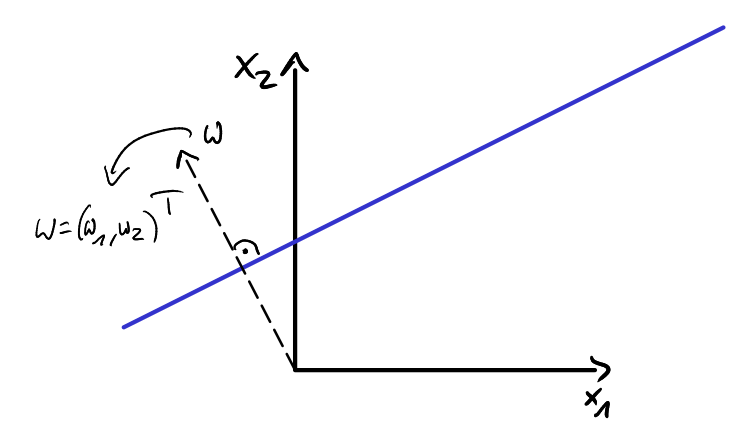
\includegraphics[width=0.7\linewidth]{sketch_7}
	\label{fig:sketch7}
\end{figure}

\paragraph{\underline{Question:}} What is the VC-dimension of
\begin{align*}
	&F =  \{ x \mapsto sign(\langle w,x \rangle): w \in \mathbb{R}^d \}\\
	&VC(F) = ?
\end{align*}

\begin{claim}$VC(F) = \textcolor{red}{d}$\end{claim}

\begin{proof}

\underline{1. We show that $VC(F)\geq d$ (lower bound):}\\
\newline
	$X = \{ c_1, ..., c_d \}$ with $c_i \in \mathbb{R}^d$ for all $i \in \{ 1, ..., d \}$\\
	$c_1 = \left(\begin{array}{c} 1 \\ 0 \\ \vdots \\ 0 \end{array}\right)$,
	$c_2 = \left(\begin{array}{c} 0 \\ 1 \\ \vdots \\ 0 \end{array}\right)$,
	$\hdots$, 
	$c_d = \left(\begin{array}{c} 0 \\ 0 \\ \vdots \\ 1 \end{array}\right)$, the basis vectors in $\mathbb{R}^d$\\
	\\
	Let 
	$w = \left(\begin{array}{c} 
		y_1 \\
		 \vdots \\
		 y_d \end{array}\right)
		 \begin{array}{c} 
		 	\textcolor{blue}{\text{ (label of 1st point)}}  \\
		 	\vdots \\
		 	\textcolor{blue}{\text{ (label of dth point)}}  
		 \end{array}$ 
	for any given $\underbrace{\text{labeling}}_ {\{ \pm 1 \}}$ of $c_1, \hdots, c_d$\\
	
	\underline{Notation:} $c_{ij} \hdots $ j-th coordinate of $c_i$
	
	$$
		\langle w, c_i \rangle = \sum_{j=1}^{d} w_j \cdot c_{ij} = 1 \cdot w_i = y_i 
	$$
	
	$\implies VC(F) \geq d$ (as we have found a set of size d that is shattered).\\
	

\underline{2. We will show the upper-bound $VC(F) < d+1$ via contradiction:}\\
\newline
\textcolor{red}{Assume that $d+1$ points $$X = \{ c_1, ..., c_{d+1} \}$$ are shattered by F.}\\
			
	This means that $\exists w_1, ..., w_{2^d+1}$ weight vectors that realize all $2^{d+1}$ labellings of the $d+1$ points. \\
	Getting \underline{all} "possible labellings" would look like this:

	$$
	M = \left(
	\begin{array}{cccccc}
		w_1^T \cdot c_1 & w_2^T \cdot c_1 	& \hdotsfor{3}						& w_{2^{d+1}}^T \cdot c_{1} \\
		w_1^T \cdot c_2 & w_2^T \cdot c_2 	& \ddots	& 			&			& w_{2^{d+1}}^T \cdot c_{2} \\
		w_1^T \cdot c_3 & w_2^T \cdot c_3 	&  			& \ddots	& 			& w_{2^{d+1}}^T \cdot c_{3} \\
		\vdots 			& \vdots 			&   		&  			& \ddots	& \vdots	\\
		w_1^T \cdot c_{d+1} & w_2^T \cdot c_{d+1} & \hdotsfor{3} 				& w_{2^{d+1}}^T \cdot c_{d+1}
	\end{array}\right)
	$$
	
	We can also write this as $XW$:
	$$
		X = \left(\begin{array}{ccc}
			\hdots & c_1 & \hdots \\
			 \hdots & c_2 & \hdots\\
			 \vdots & \vdots & \vdots \\
			\hdots & c_1 & \hdots
		\end{array}\right), 
		W = \left(\begin{array}{cccc}
			\vdots & \vdots & \vdots & \vdots \\
			w_1 & w_2 & \hdots & w_{2^{d+1}}\\
			\vdots & \vdots & \vdots & \vdots
		\end{array}\right)
	$$
	Taking $\text{sign}(XW)$ componentwise gives \underline{all} possible labellings. Let \textcolor{red}{$M = XW$}.\\
	We know that 
	\begin{align*}
		\text{rank}(M) \leq \min\{ \text{rank}(X), \text{rank}(W) \} \text{\textcolor{red}{$= d$}} & \hspace{1cm} \text{(by virtue of rank$(\cdot)$)}
	\end{align*}
	
 \paragraph{Claim:} Under the shattering assumption, the rows of M are linearly independent!
 $$ \alpha_1 v_1 + \hdots + \alpha_n v_n = \vec{0}$$
 \newline
 \textcolor{red}{ Hier Matrix M nochmal einfügen}
 \newline
\begin{align*}
a_1 \cdot \text{row}_1 + \hdots + a_n \cdot \text{row}_n &=\\
a_1 \cdot ( w_1^T \cdot c_1, w_2^T\cdot c_1, \hdots, w_{2^{d+1}}^T\cdot c_1 ) &+\\
a_2 \cdot ( w_1^T\cdot c_2, w_2^T\cdot c_2, \hdots, w_{2^{d+1}}^T\cdot c_2 ) &+\\
\hdots &+\\
a_{d+1} \cdot ( w_1^T \cdot c_{d+1}, w_2^T\cdot c_{d+1}, \hdots, w_{2^{d+1}}^T\cdot c_{d+1} ) &=
\end{align*}

\begin{align*}
	\vec{x} = (a^T X w_1, a^T X w_2, \hdots, a^T X w_{2^{d+1}}) \textcolor{red}{=^? \vec{0}}
\end{align*}
\textcolor{red}{hier einfügen}
\newline
Fact is, due to the shattering assumption, there is a \textcolor{red}{k} such that

$$
	\text{sign}(a) = \text{sign}(Xw_{\textcolor{red}{k}})
$$
$$
\Rightarrow a^T X w_{\textcolor{red}{k}} \text{ is positive}
$$
$\Rightarrow$ The all zeros vector can only be achieved if all $a_i$ are 0\\
$\Rightarrow$ we have d+1 independent rows $\Rightarrow \text{rank}(M) = d+1$\\
BUT, $\text{rank}(M) \leq d$! $\Rightarrow$ Contradiction (meaning our assumption is wrong). Consequently, $VC(F) < d+1$ and with $VC(F) \leq d$ we obtain $$\textcolor{red}{VC(F) = d}$$
\end{proof}


\paragraph{Example:} Learning halfspace classifiers\\
$$\text{HS}_d = \{ x \mapsto h_{w,b}(x), h_{w,b} \in L_d \}$$
we are only looking at the \underline{realizable case}.
$$S = ((x_1, y_1), ..., (x_m, y_m));\  \ y_i \in {\pm 1}$$

ERM on $\text{HS}_d$ means to find \textcolor{blue}{$w \in \mathbb{R}^{d}$}, such that 
$$
\forall i \in \{ 1, ..., m \}: \text{sign}(\langle \textcolor{blue}{w}, x_i\rangle) = y_i
$$
or equivalently 
$$
y_i =  \langle \textcolor{blue}{w}, x_i\rangle > 0 \forall i \in \{ 1, ..., m \}
$$

\textcolor{red}{hier Bild einfügen}

Letting $$\overline{w} =  \frac{w^*}{\gamma}$$ we have 
$$
	\forall i \in \{ 1, ..., m \}: y_i \langle \overline{w}, x_i\rangle = y_i \langle \frac{w^*}{\gamma}, x_i \rangle = \frac{1}{\gamma} \cdot y_i \langle w^*, x_i \rangle \geq 1
$$

This shows that a vector $w \in \mathbb{R}^{d}$ with
$$
	\forall i: y_i \langle w, x_i \rangle \text{ has to exist! (**)}
$$

We can write (**) as \textcolor{blue}{$Aw \geq v$} with \\
\textcolor{red}{ matrix hier einfügen}\\
A \underline{linear program} (LP) is
$$
	\underbrace{\max_{w \in \mathbb{R}^{d}} \langle u, w \rangle}_{\text{\textcolor{blue}{linear objective}}} \text{ subject to } 
	\underbrace{Aw \geq v}_{\textcolor{blue}{\text{linear constraints}}}
$$ 
Take $u \in \mathbb{R}^{d}$ as, e.g., $u = (1, \hdots, 1)^T$ 

\part{Rademacher Complexity}
In short: RC is the ability of a class to correlate well with random noise.\\
RC can be bounded by the growth function or the VC-dim bounds. RC can be tighter than the VC-dim. bounds!\\
\underline{Conventions:} $H$, a hypothesis class; $l: H\times Z \to \mathbb{R}$, a loss function; to each $h \in H$, we associate a function g ($ g \in G$) that maps $(x,y) \mapsto l(h, (x,y)) $ (i.e. tuple x,y is mapped to its loss).\\
\newline
E.g.: $G = \{ (x,y) \mapsto \underbrace{\mathbbm{1}_{h(x) \neq y}}_{\text{0-1 loss}}: h\in H \}$

\begin{boxeddef}[Empirical Rademacher complexity]
	Let $G$ be a class of functions from $Z = X \times Y$ to $[a, b]$ and $\mathbb{S} = (z_1, ..., z_n)$ with $z_i \in Z$. Then, the empirical Rademacher complexity is defined as:
	$$
		\hat{R_s}(G) = \mathbb{E}_\sigma\bigg[\sup_{g \in G} \frac{1}{m} \cdot \sum_{i = 1}^{m} \sigma_i g(z_i)\bigg]
	$$
	with $\sigma = (\sigma_1, ..., \sigma_m)^T$, $\sigma_i \sim^{iid} \text{ uniform}\left(\{ \pm 1 \}\right)$
\end{boxeddef}

\begin{boxeddef}[Rademacher complexity]
	Let $\mathcal{D}$ be a distribution over $Z = X \times Y$. For any $m \geq 1$, the Rademacher complexity of G is defined as
	$$
		R_m(G) = \mathbb{E}_{S \sim \mathcal{D}^m} \big[\hat{R_s}(G)\big]
	$$
\end{boxeddef}

\paragraph{Theorem:} Let G be a class of functions from $Z$ to $[0,1]$. For any $\delta > 0$, we have with probability of at least $1-\delta$, that (1) and (2) hold for all $g \in G$:
\begin{enumerate}
	\item $\mathbb{E}_z \big[g(z)\big] \leq \frac{1}{m} \cdot \sum_{i = 1}^{m} g(z_i) + 2 R_m (G) + \sqrt{\frac{\log(\frac{1}{\delta})}{2m}}$
	\item $\mathbb{E}_z \big[g(z)\big] \leq \frac{1}{m} \cdot \sum_{i = 1}^{m} g(z_i) + 2 \hat{R_s} (G) + 3 \cdot \sqrt{\frac{\log(\frac{2}{\delta})}{2m}}$
\end{enumerate}
\textcolor{blue}{(2) is a "data-dependent" bound (via S)!}
\begin{proof}
	For any $S = (z_1, ..., z_m)$ and any $g \in G$, let
	$$
		\hat{\mathbb{E}_s}[g] = \frac{1}{m} \sum_{i = 1}^{m} g(z_i)
	$$
	Let \textcolor{blue}{$$\phi(s) = \sup_{g \in G} \mathbb{E}[g] - \hat{\mathbb{E}_S}[g]$$}. Also, let $S, S'$ be \underline{two} samples that only differ in one instance, e.g. $z_i$ in $S$ and $z_{i}'$ in $S'$.
	\begin{align*}
		\phi(S')-\phi(S) &= \sup_{g \in G} \mathbb{E}[g] - \hat{\mathbb{E}_S'}[g] - sup_{g \in G} \mathbb{E}[g] - \hat{\mathbb{E}_S}[g]\\
		&\leq  \sup_{g \in G} \hat{\mathbb{E}_{\textcolor{blue}{S}}}[g] - \sup_{g \in G} \hat{\mathbb{E}_{\textcolor{red}{S'}}}[g]\\
		&= \sup_{g \in G} \frac{g(z_i) - g(z_{i}')}{m} \leq \frac{1}{m}
	\end{align*}
	\colorbox{orange}{hier ergänzen}
\end{proof}

\begin{boxeddef}[McDiarmid inequality]
	Let $X_1, ..., X_m$ be $m \geq 1$ independent random variables and assume that there exist $c_y, ..., c_m > 0$ such that $f: \mathcal{X}^m \to \mathbb{R}$ satisfies:
	$$
		\bigg|f(x_1, \hdots , x_i, \hdots, x_m) - f(x_1, \hdots, x_{i}', \hdots, x_m) \bigg| \leq c_i \ \ \forall i \in \{ 1, ..., m \}
	$$
	Remark: $\mathcal{X}^m = \underbrace{\mathcal{X} \times \mathcal{X} \times ... \times \mathcal{X}}_{\text{m-times}}$\\
	
	for any $x_1, ..., x_m, x_{i}' \in \mathcal{X}$. Let $f(S)$ denote $f(X_1, ..., X_m)$. Then, for all $\varepsilon > 0$:
	\begin{enumerate}
		\item $\mathbb{P}[f(s) - \mathbb{E}[f(S)] \geq \varepsilon] \exp (\frac{-2\varepsilon^2}{})$
		\colorbox{orange}{hier ergänzen}
	\end{enumerate}
\end{boxeddef}

	By McDiarmid's inequality, we have (with $c_i = \frac{1}{m}$)
	$$
		\mathbb{P}[\phi(S) - \mathbb{E}[\phi(S)] \geq \varepsilon] \leq \underbrace{\exp \bigg(\frac{-2\varepsilon^2}{\sum_{i} \frac{1}{m^2} }\bigg)}_{\text{let this be $<\delta$ and express $\varepsilon > \sqrt{ \frac{\log(\frac{1}{\delta})}{2m} }$}}
	$$
	$$
	\Rightarrow \phi(S) - \mathbb{E}_S[\phi(S)] \leq \sqrt{\frac{1}{2m} \cdot \log(\frac{1}{\delta})}
	$$
	holds with probability of at least $1-\delta$.\\
	OR\\
	$$
		\phi(S) \leq \mathbb{E}_s[\phi(S)] + \sqrt{\frac{1}{2m} \cdot \log(\frac{1}{\delta})}
	$$
	Now look at that first term:
\begin{align*}
		\mathbb{E}_s[\phi(S)] &= \mathbb{E}_s \big[\sup_{g \in G} \mathbb{E}[g] - \hat{\mathbb{E}_{S}}[g]\big]\\
		&\ \ \ \text{with: } \mathbb{E}_{S'}[\hat{\mathbb{E}_{S'} [g]}] = \mathbb{E}[g]\\
		&= \mathbb{E}_S \bigg[ \sup_{g \in G} \mathbb{E}_{S'} \big[  \hat{\mathbb{E}_{S'}} [g] - \hat{\mathbb{E}_{S}} [g] \big] \bigg]\\
		&\leq \mathbb{E}_{S,S'} \bigg[ \mathbb{E}_{S'} \sup_{g \in G}\big(  \hat{\mathbb{E}_{S'}} [g] - \hat{\mathbb{E}_{S}} [g]\big) \bigg]\\
		&= \mathbb{E}_{S,S'}\bigg[ \sup_{g \in G} \bigg( \frac{1}{m} \cdot \sum_{i_1}^{m} g(z_{i}') - g(z_i)\bigg) \bigg]\\
		&= \mathbb{E} \bigg[ \sup_{g \in G} \bigg( \frac{1}{m} \cdot \sum_{i_1}^{m} \sigma_i \big( g(z_{i}') - g(z_i) \big)  \bigg)  \bigg]\\
		& \text{Remark: We know $ \sup(A+B) \leq \sup(A) + \sup(B)$}\\
		&= \mathbb{E}_{\sigma, S, S'}\bigg[ \sup_{g \in G} \bigg( \frac{1}{m} \cdot \sum_{i_1}^{m} \sigma_i  g(z_{i}')  + \frac{1}{m} \cdot \sum_{i_1}^{m} \sigma_i \cdot -g(z_{i})  \bigg)  \bigg]\\
		&\leq \mathbb{E}_{\sigma, S'}\bigg[ \sup_{g \in G} \bigg( \frac{1}{m} \cdot \sum_{i_1}^{m} \sigma_i g(z_{i}') \bigg) \bigg] +
		\mathbb{E}_{\sigma, S}\bigg[ \sup_{g \in G} \bigg( \frac{1}{m} \cdot \sum_{i_1}^{m} -\sigma_i g(z_{i})  \bigg) \bigg]\\
		&= \textcolor{red}{2} \cdot \mathbb{E}_{\sigma, S}\bigg[ \sup_{g \in G} \bigg( \frac{1}{m} \cdot \sum_{i_1}^{m} \sigma_i \cdot g(z_{i})  \bigg) \bigg] \\
		&= 2 \cdot R_m(G)
\end{align*}

\end{document}